\documentclass[slidestop, compress, mathserif]{beamer}
\usepackage[style=authoryear-comp, sorting=nyt, maxcitenames=2, backend=biber]{biblatex}
\renewbibmacro{in:}{}
\renewcommand\bibfont{\small}
\addbibresource{ref_01.bib}
\addbibresource{ref_02.bib}
\addbibresource{ref_03.bib}
\addbibresource{trappe.bib}

\usepackage{amsmath, amssymb, mathrsfs}
\usepackage{color, graphicx}

\usepackage{setspace, listings}
\usepackage{sidecap}

\usetheme{Madrid}
\usecolortheme{default}
\linespread{1.2}



\sidecaptionvpos{figure}{c}
\usepackage[textfont=small]{caption}
\setbeamertemplate{caption}[numbered]
\captionsetup{font=scriptsize, labelfont=scriptsize, labelformat=simple}

\setbeamertemplate{footline}
{
  \leavevmode%
  \hbox{%
  \begin{beamercolorbox}[wd=1.0\paperwidth,ht=2.25ex,dp=1ex]{author in head/foot}\usebeamerfont{author in head/foot}
    \hspace*{3ex}
    \inserttitle
    \hfill
    \insertshortauthor
    \hspace*{3ex}
  \end{beamercolorbox}%
}%
  \vskip0pt%
}


\title{Simulation in Equilibrium}
\author{Gun Woo Park}
% \institute{DICMaPI, University of Naples Federico II}
% \author{Gun Woo Park, Antonio Brasiello, and Giovanni Ianniruberto}
% \date{SUPOLEN PROJECT MEETING\\ 27 MAR 2015}


% it's for headline
% \setbeamertemplate{headline}{%
%   % \leavemode%
%   \hbox{%
%     % \begin{beamercolorbox}[wd=\paperwidth,ht=2.5ex,dp=1.125ex]{palette quaternary}%
%     \begin{beamercolorbox}[wd=\paperwidth,ht=2.5ex,dp=1.125ex]{section in head/foot}%
%       \insertsectionnavigationhorizontal{\paperwidth}{}{\hskip0pt plus1filll}
%     \end{beamercolorbox}%
%     }
% }

\begin{document}

\begin{frame}[plain]
\maketitle
\end{frame}

% \begin{frame}
%   \frametitle<presentation>{Preliminary}
%   \vspace{-0.15in}
%   \begin{block}{Instantaneous Pressure Function}
%     Let $\mathscr{P} = \left[\mathscr{P}_{ij}\right]$ be a deviatoric part for isotropic instantaneous pressure function is given by the virials:
%     \vspace{-0.2in}
%     \begin{equation}
%       V\mathscr{P} = \sum_{i=1}^{N_{tot}} \mathbf{r}_i\mathbf{F}_i,
%     \end{equation}
%     where $N_{tot}$ be the number of total chains in the box, $\mathbf{r}_i$ be the relative position vector for i-th chain in the system (i.e., connector vector for the chain), and $\mathbf{F}_i$ be a force exerted on the subjected chain. 
%   \end{block}
%     Because the instantaneous stress tensor is given by $-\mathscr{P}$, we have
%   \begin{equation}
%     \tau_{xy} = -\frac{1}{V}\sum_{i=1}^{N_{tot}} x\left[\mathbf{r}_i\right]y\left[\mathbf{F}_j\right].
%   \end{equation}
% \end{frame}

% \begin{frame}
%   \frametitle<presentation>{Preliminary (cont.)}
%   \begin{block}{Shear Relaxation Modulus and Viscosity}
%     For given instantaneous shear stress, $\tau_{xy}$, the shear relaxation modulus is given by its autocorrelation function (ACF), $C$:
%     \begin{equation}
%       G(t) = C_{\tau_{xy}}(t).
%     \end{equation}
%     The shear viscosity is expressed by
%     \begin{equation}
%       \eta = \frac{V}{k_BT} \int_{0}^{\infty} G(t) dt.
%     \end{equation}
%   \end{block}
% \end{frame}

% \begin{frame}
%   \frametitle<presentation>{Autocorrelation Function}
%   \begin{block}{Basics for Correlation Function}
%     The correlation function between two time dependent functions, $f$ and $g$, are given by
%     \begin{equation}
%       Corr[f, g] = \langle f(\xi)g(\xi + t) \rangle_{\xi},
%     \end{equation}
%     where $\langle \cdots \rangle_{\xi}$ denote average over $\xi$.
%   \end{block}
%   The autocorrelation function, $C_f$, (without normalization) is given by
%   \begin{equation}
%     C_f(t) = Corr[f, f](t) \left( \equiv \langle f(\xi)f(\xi + t) \rangle_{\xi} \right).
%   \end{equation}
% \end{frame}

% \begin{frame}
%   \begin{block}{Practical Form for Discrete ACF}
%     Let the time is discretized based on time index, $i$ and $j$, the practical form for ACF is given by
%     \begin{equation}
%       C_f(i\Delta t) = \frac{1}{N-i}\sum_{j=0}^{N-i-1}f(j\Delta t)f((i+j)\Delta t)
%     \end{equation}
%     where $N$ is maximum number and $\Delta t$ is time between each time index.
%   \end{block}
%   It is frequently used the same time lag for the ACF by
%   \begin{equation}
%     C_f(i\Delta t) = \frac{1}{N-M}\sum_{j=0}^{N-M-1}f(j\Delta t)f((i+j)\Delta t)
%   \end{equation}
%   with $M\leq N/2$.
% \end{frame}

% \begin{frame}
%   \begin{block}{ACF for Correlated Data}
%     Let $K\Delta t$ be the fully uncorrelated time for given $f(t)$, the ACF using block average is expressed by
%     \begin{equation}
%       C_f(i\Delta t) = \frac{1}{N_B}\sum_{j=0}^{N_B - 1}f(jK\Delta t)f((i+jK)\Delta t),
%     \end{equation}
%     where $N_B \leq \frac{N/2}{K}$.
%   \end{block}
% \end{frame}

% \begin{frame}
%   \frametitle<presentation>{Effect of Time Step for Brownian Motion}
%   \begin{figure}
%     \centering
%     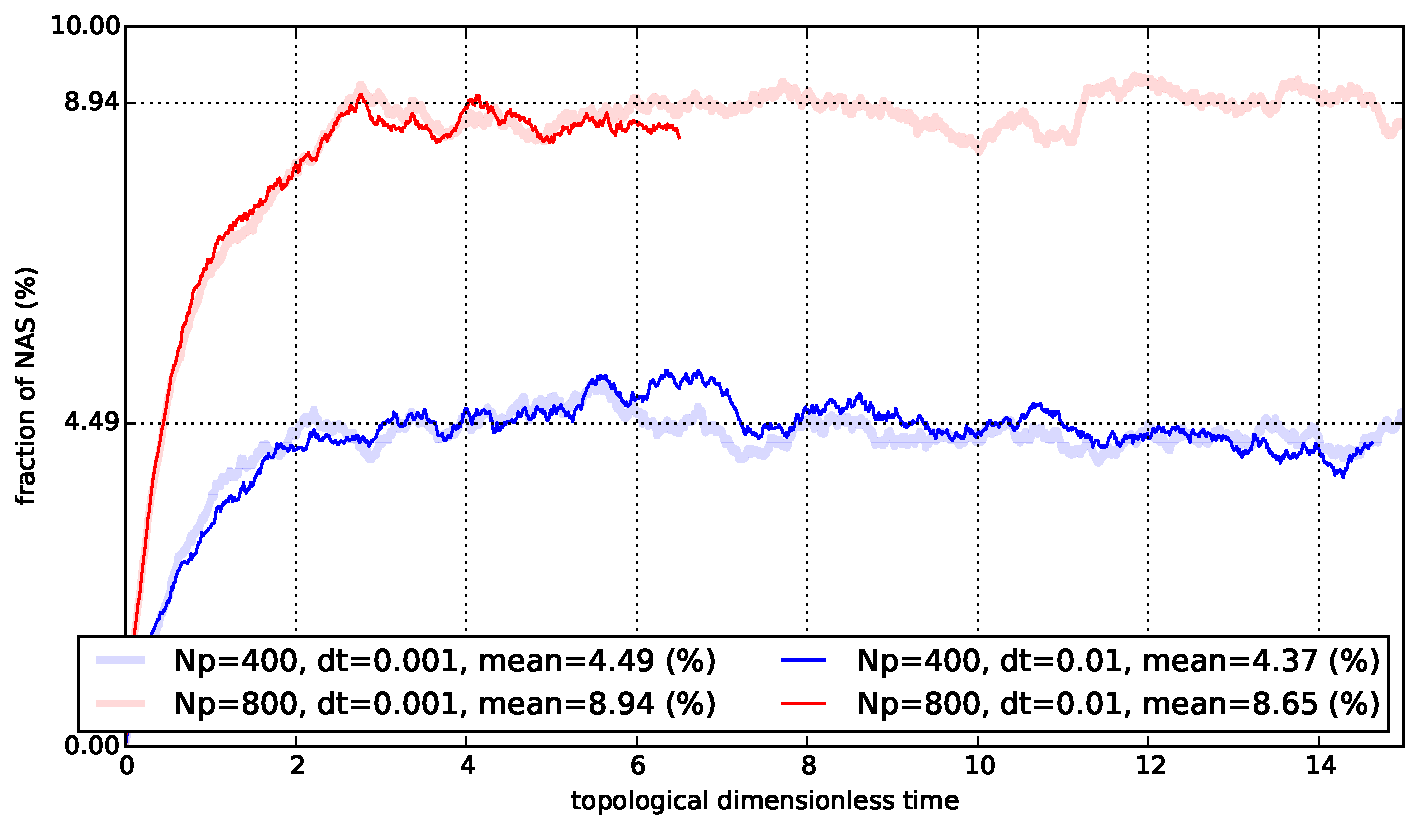
\includegraphics[width=\textwidth]{../check_time_step.pdf}
%   \end{figure}
% \end{frame}

\begin{frame}
  \frametitle<presentation>{Average detachment frequency and correlation time}
  \begin{figure}
    \centering
    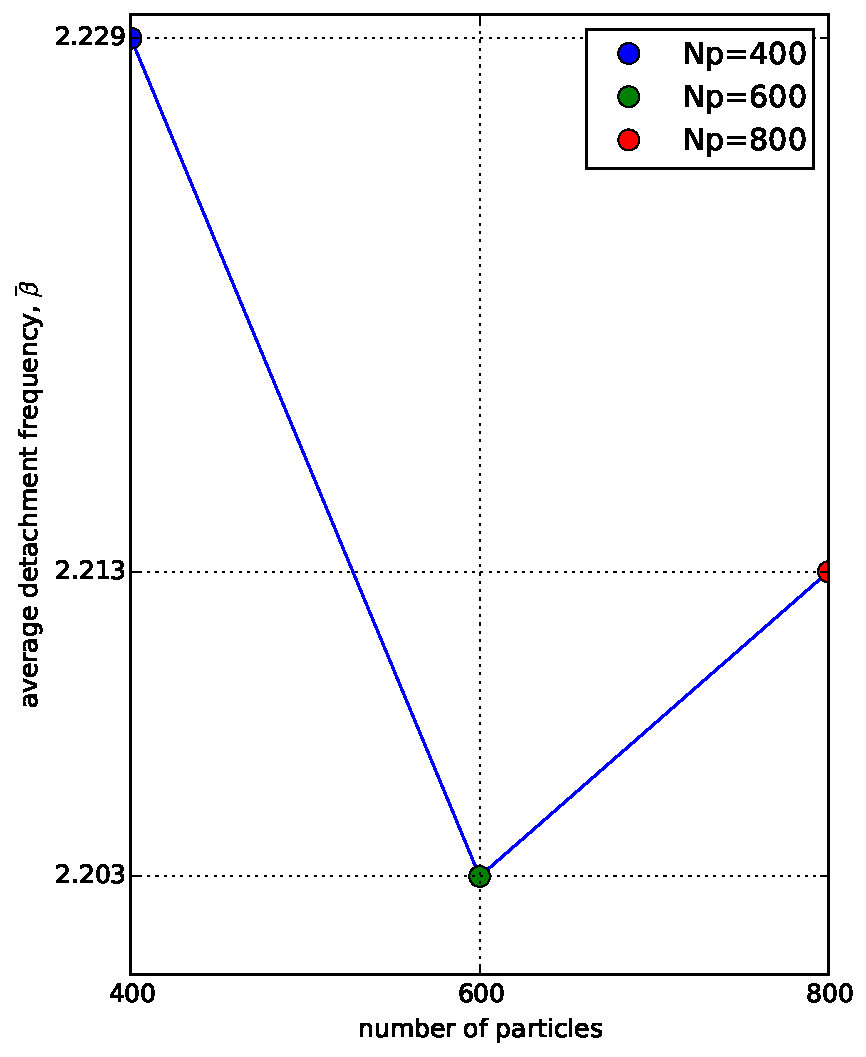
\includegraphics[width=0.33\textwidth]{../check_beta.pdf}
    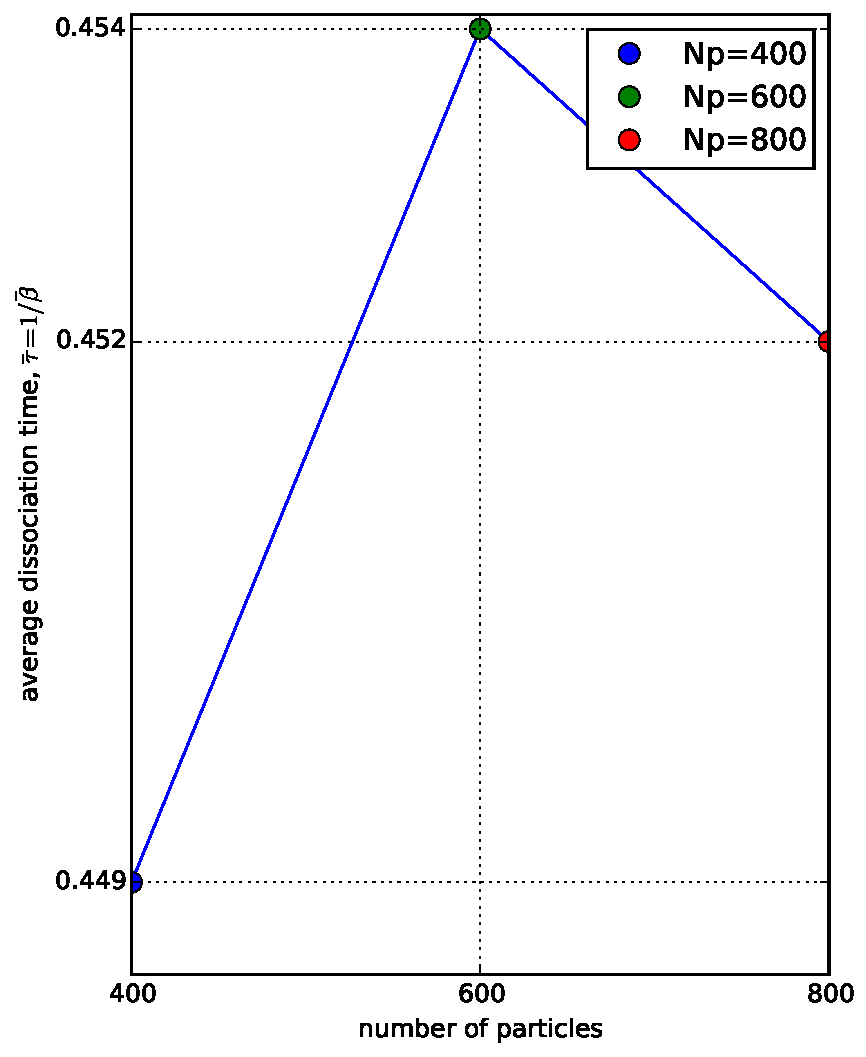
\includegraphics[width=0.33\textwidth]{../check_tau.pdf}
    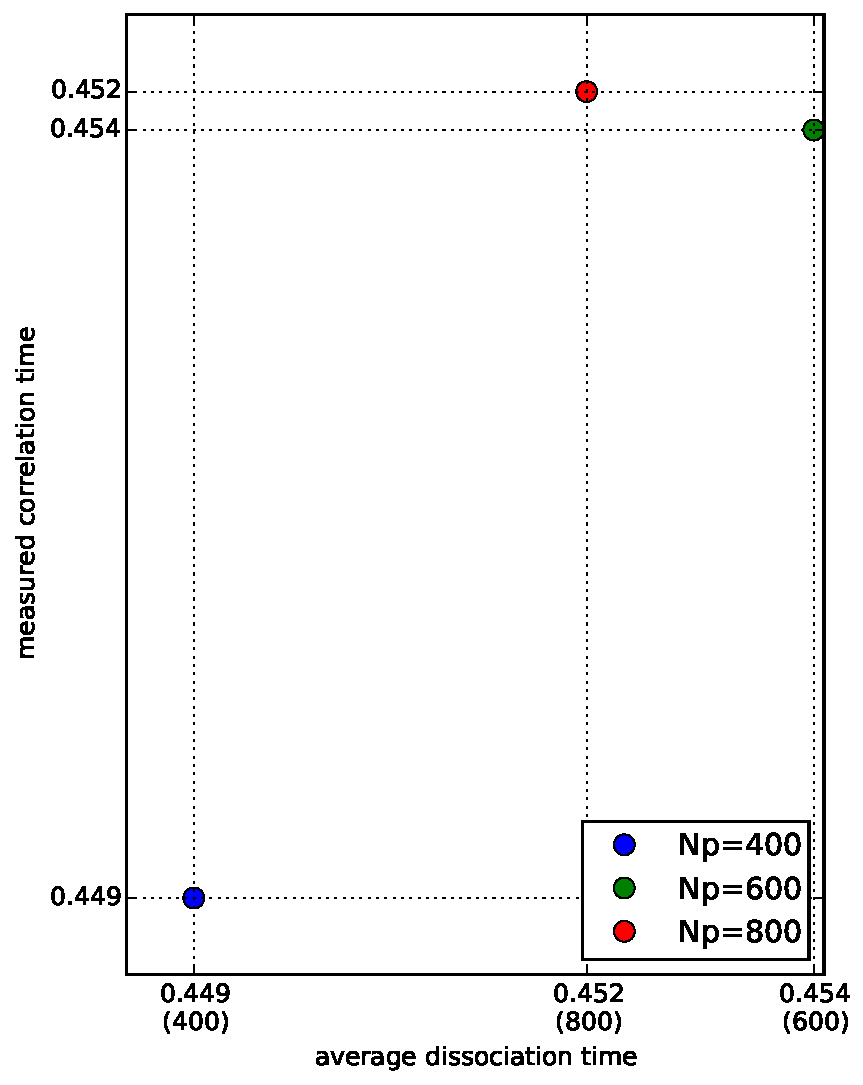
\includegraphics[width=0.33\textwidth]{../correlation_time_tau.pdf}
    \caption{Average detachment frequency (left) and average dissociation time (center), and the correlation time with respect to average dissociation time (right). The correlation time for NP=800 case is regarded as poor statistics which will be checked tomorrow.}
  \end{figure}
\end{frame}

\begin{frame}
  \frametitle<presentation>{Check Equilibrium}
  \begin{figure}
    \centering
    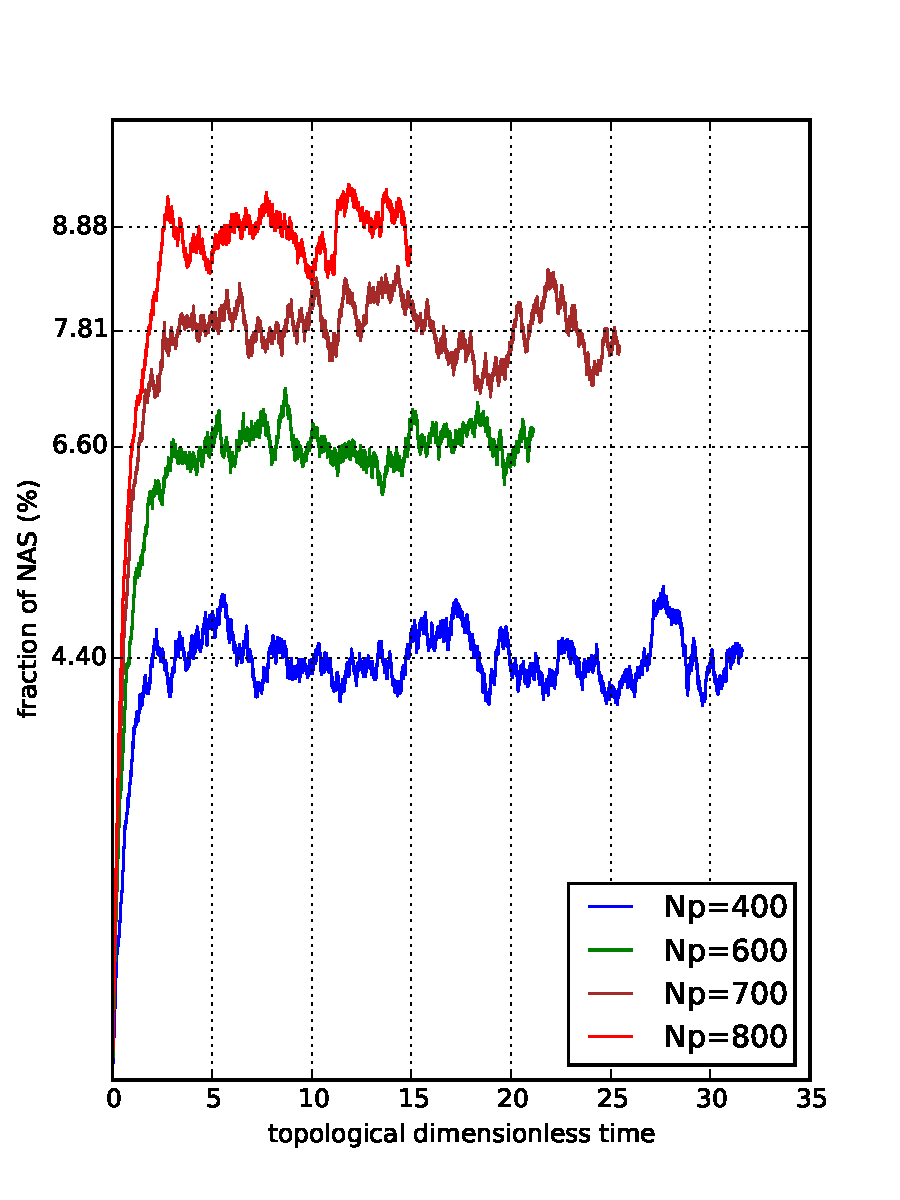
\includegraphics[width=0.4\textwidth]{../check_equilibrium_refined.pdf}
    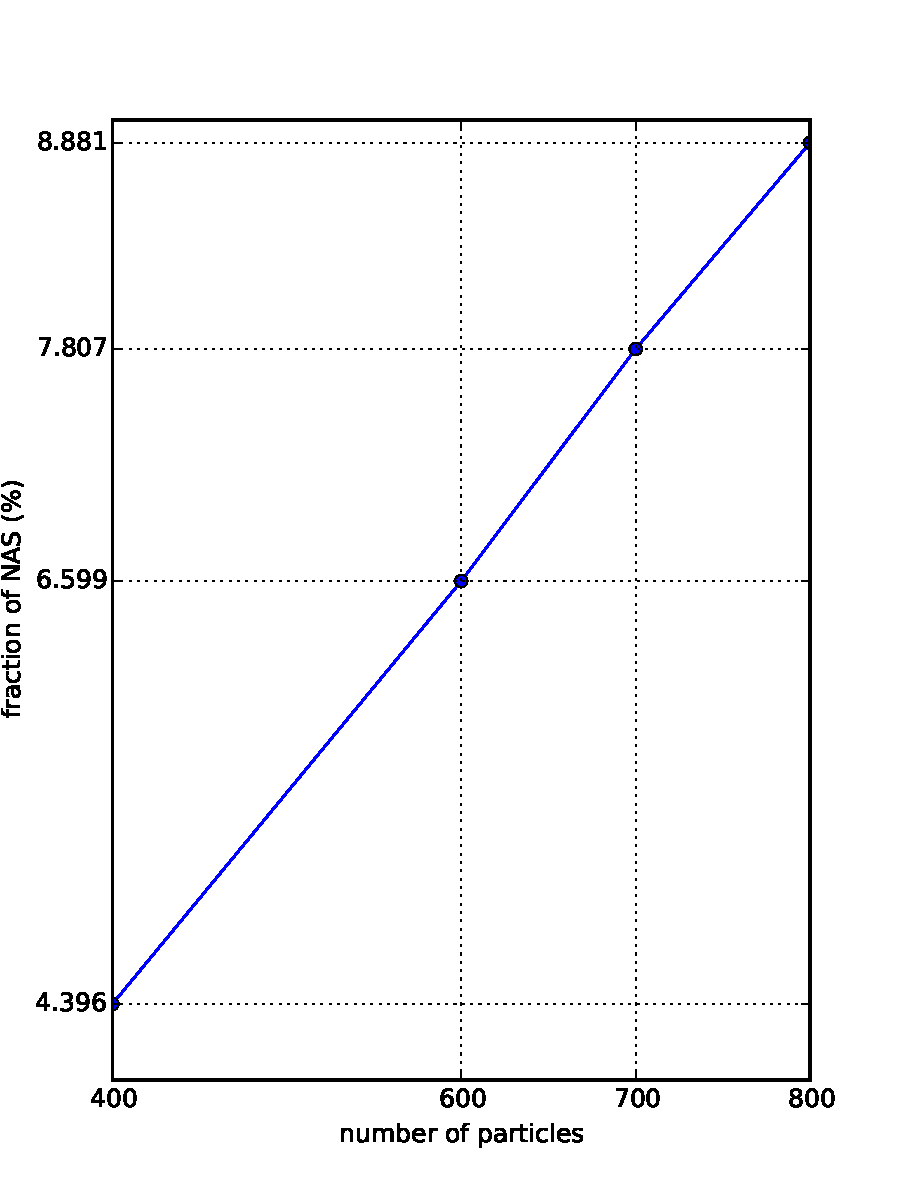
\includegraphics[width=0.4\textwidth]{../check_fNAS.pdf}
    
  \end{figure}
\end{frame}

\begin{frame}
  \frametitle<presentation>{Shear Stress}
  \begin{figure}
    \centering
    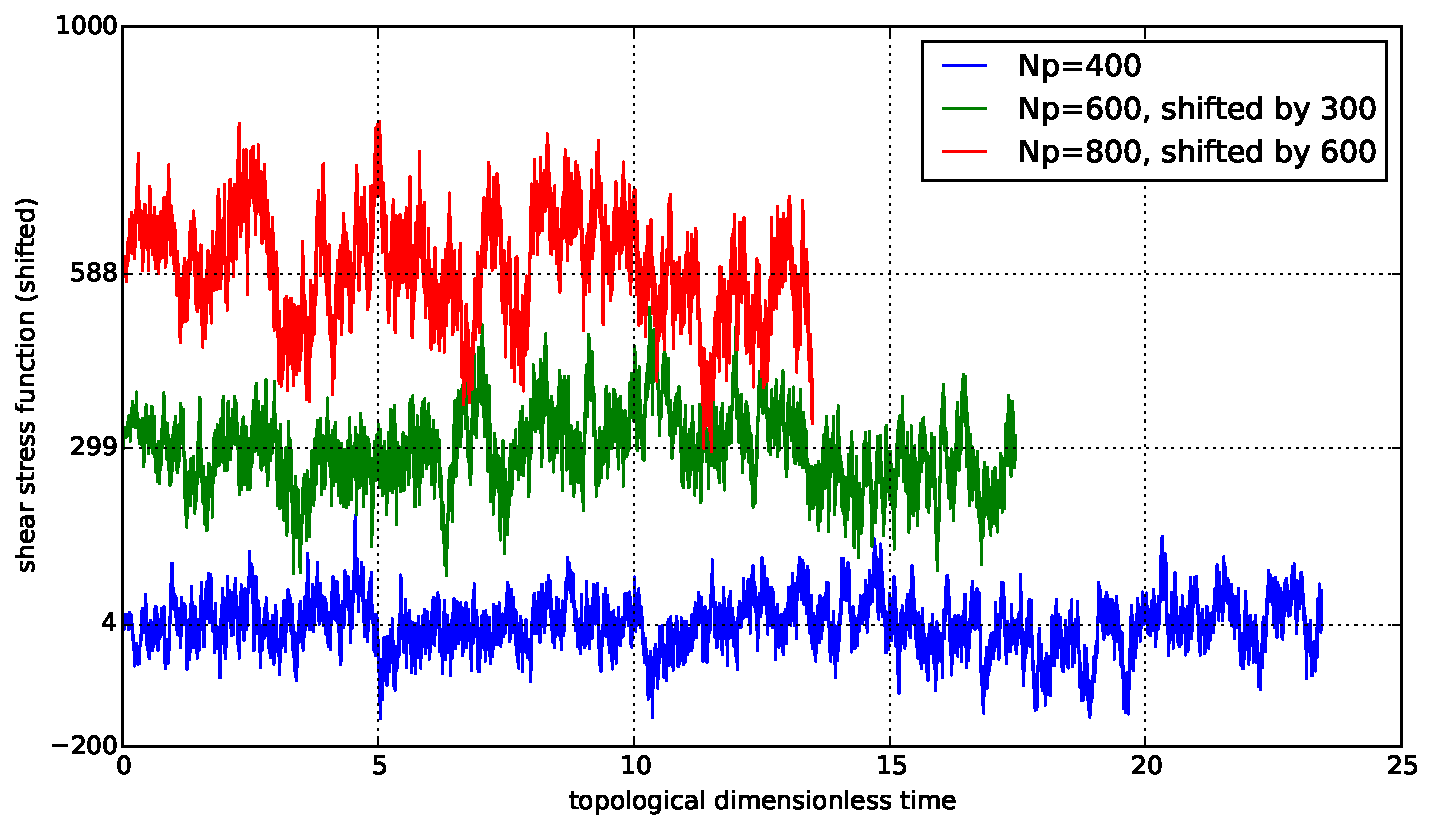
\includegraphics[width=\textwidth]{../check_shear_stress.pdf}
  \end{figure}
\end{frame}

\begin{frame}
  \frametitle<presentation>{Check ACF, linear}
  \begin{figure}
    \centering
    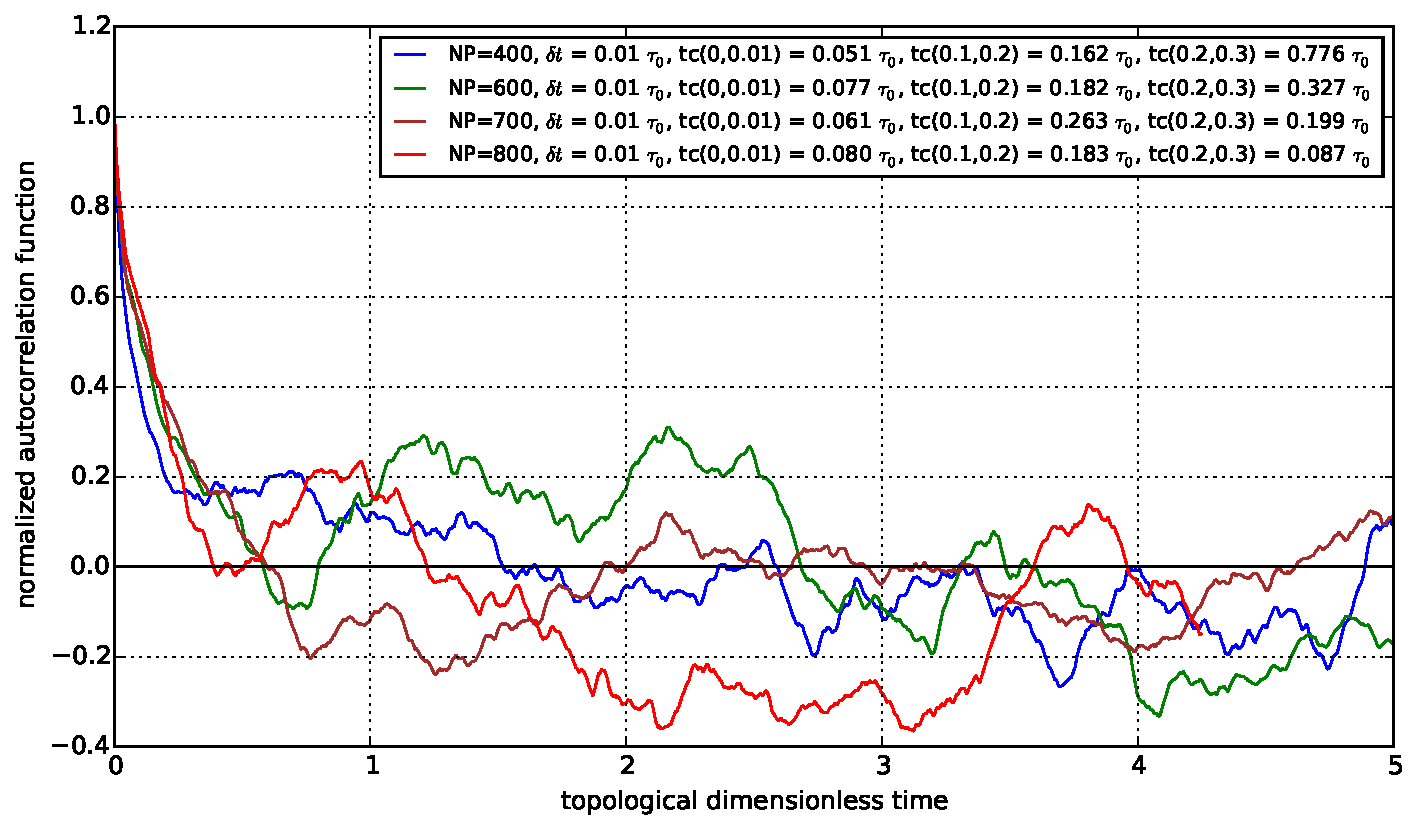
\includegraphics[width=\textwidth]{../check_ACF_initial.pdf}
  \end{figure}
\end{frame}

\begin{frame}
  \frametitle<presentation>{Check ACF, linear (short range)}
  \begin{figure}
    \centering
    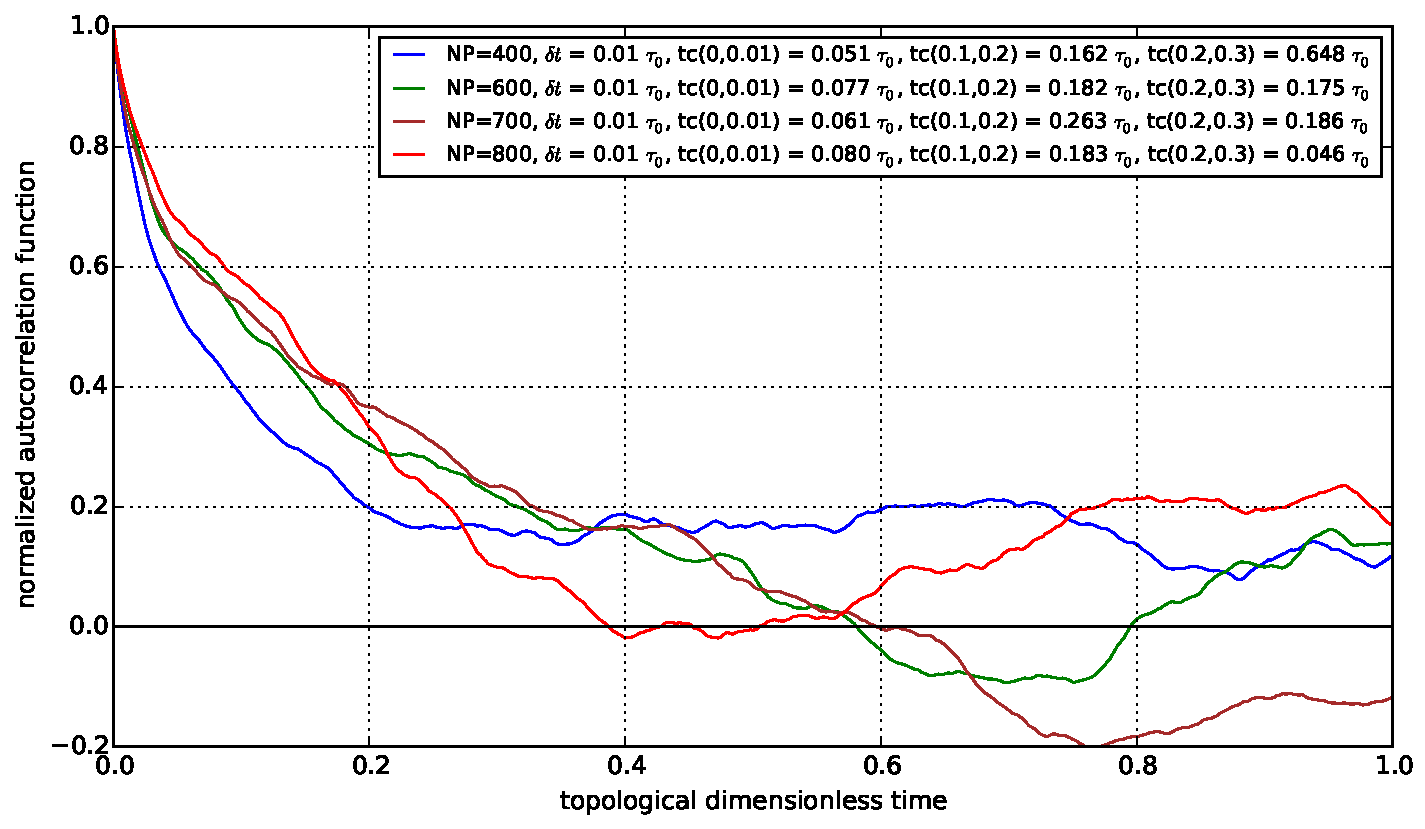
\includegraphics[width=\textwidth]{../check_ACF_initial_detail.pdf}
  \end{figure}
\end{frame}

\begin{frame}
  \frametitle<presentation>{Check ACF, semilogy}
  \begin{figure}
    \centering
    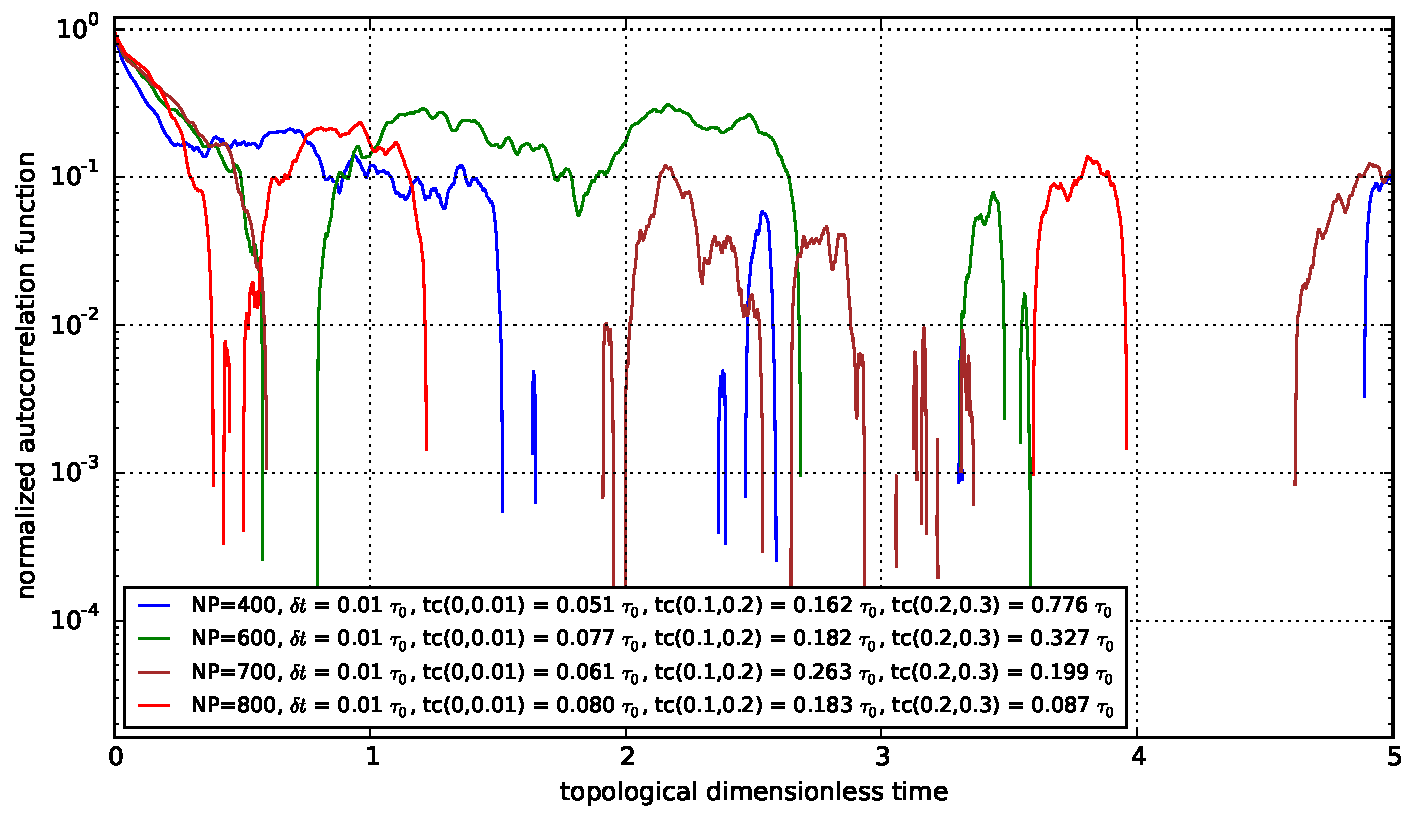
\includegraphics[width=\textwidth]{../check_ACF_initial_semilogy.pdf}
  \end{figure}
\end{frame}

\begin{frame}
  \frametitle<presentation>{Check ACF, semilogy (short range)}
  \begin{figure}
    \centering
    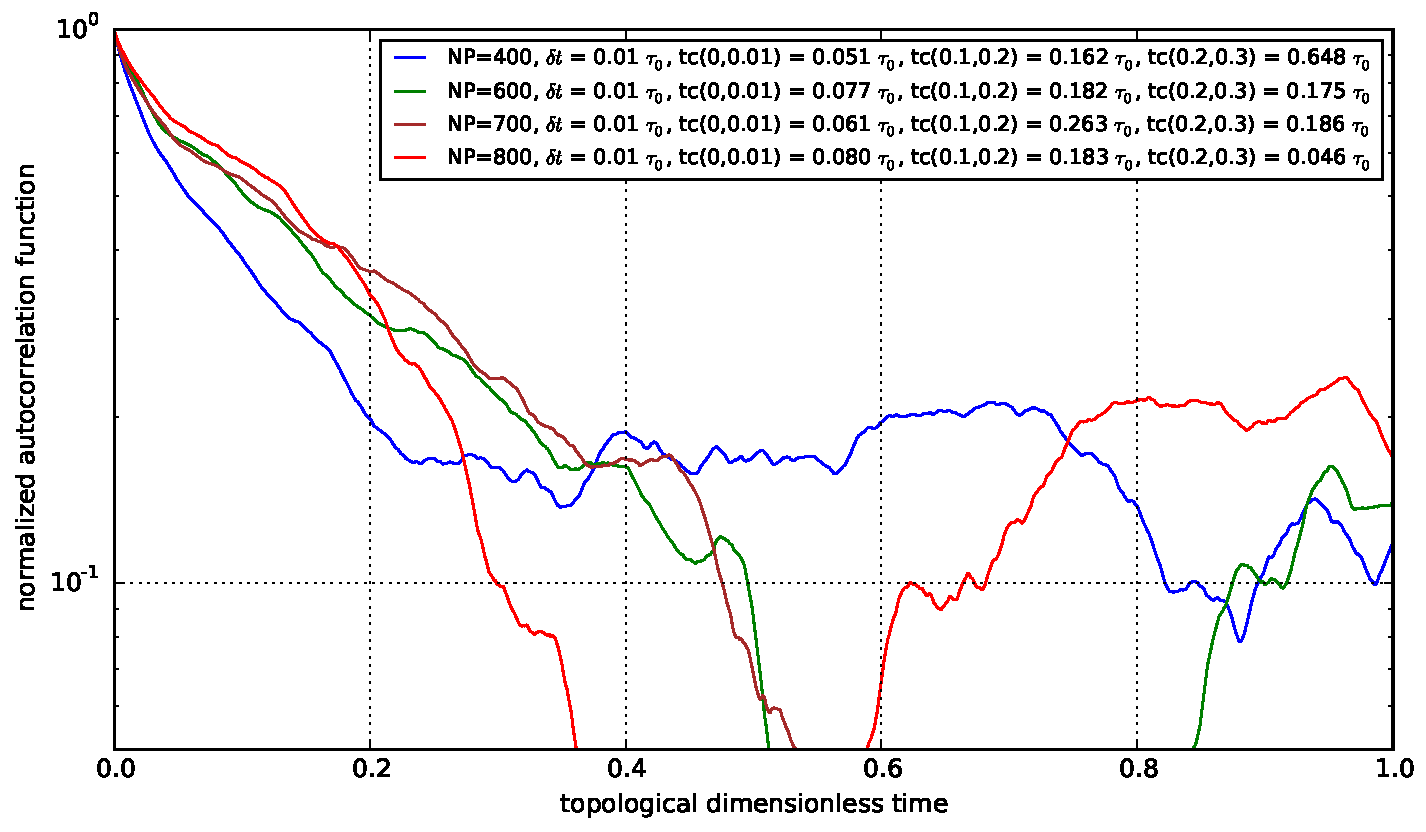
\includegraphics[width=\textwidth]{../check_ACF_initial_semilogy_detail.pdf}
  \end{figure}
\end{frame}

\begin{frame}
  \frametitle<presentation>{Check ACF, double log}
  \begin{figure}
    \centering
    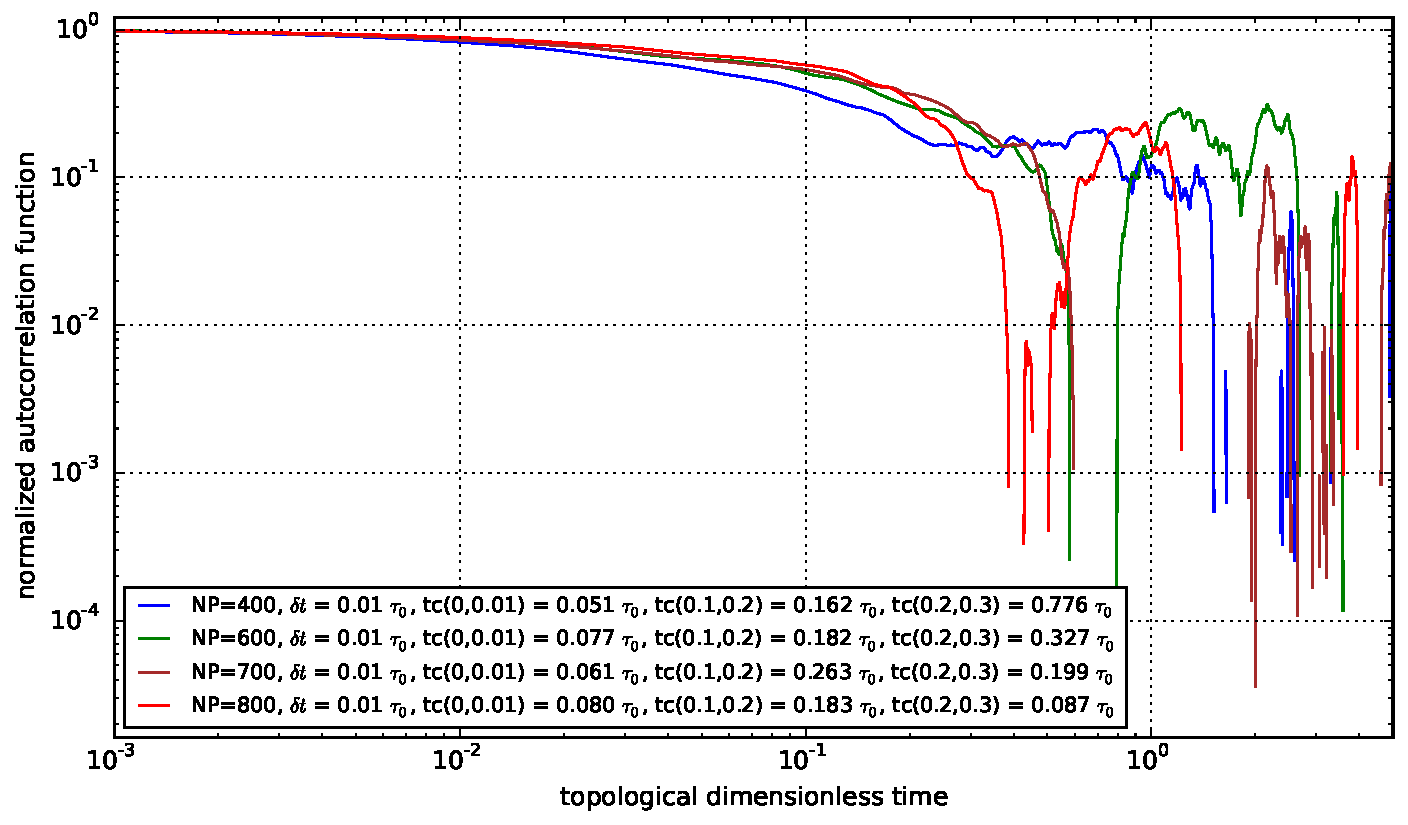
\includegraphics[width=\textwidth]{../check_ACF_initial_loglog.pdf}
  \end{figure}
\end{frame}

\begin{frame}
  \frametitle<presentation>{Check ACF, double log (short range)}
  \begin{figure}
    \centering
    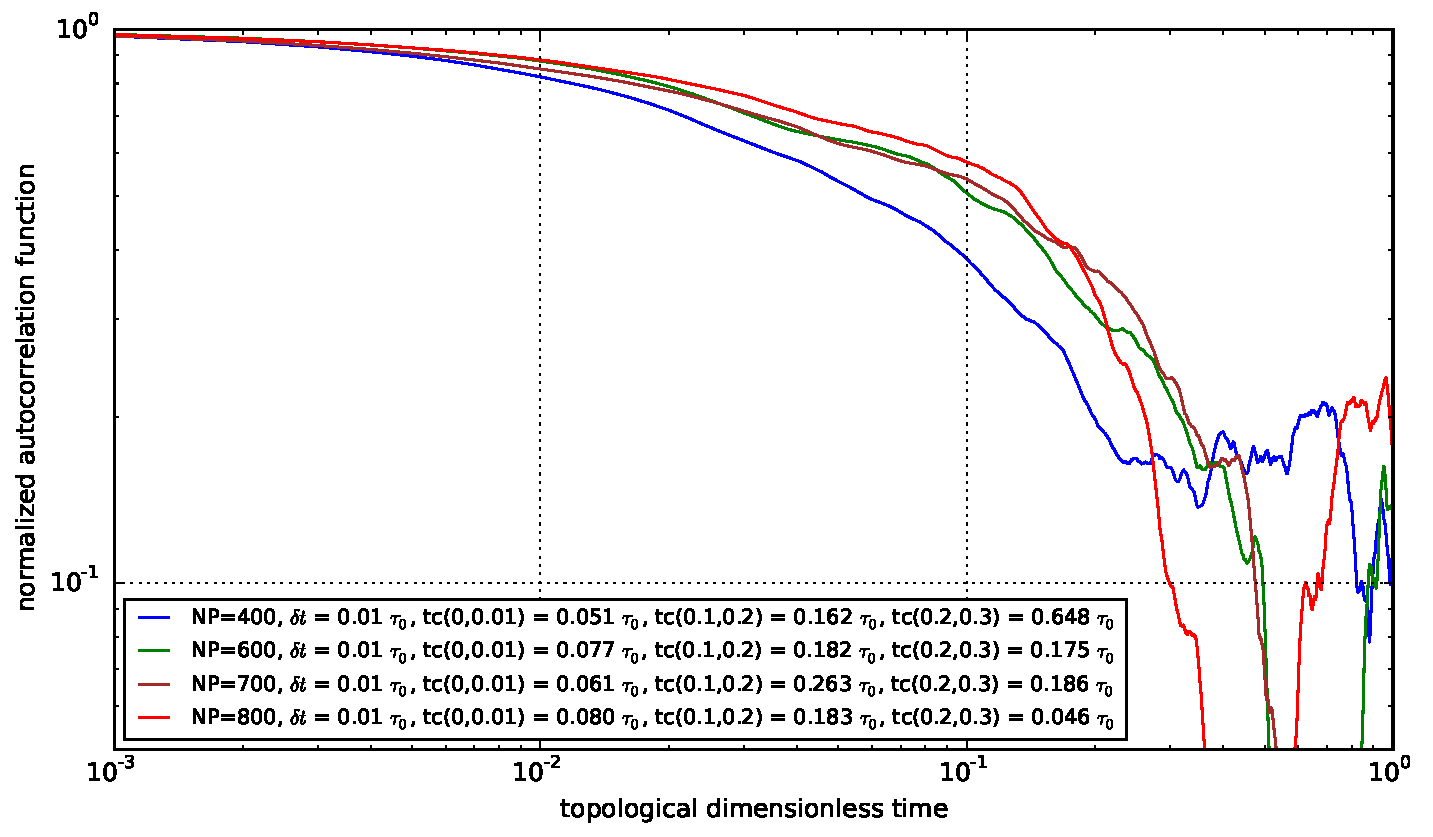
\includegraphics[width=\textwidth]{../check_ACF_initial_loglog_detail.pdf}
  \end{figure}
\end{frame}

\begin{frame}
  \frametitle<presentation>{Check Scaling Law}
  \begin{figure}
    \centering
    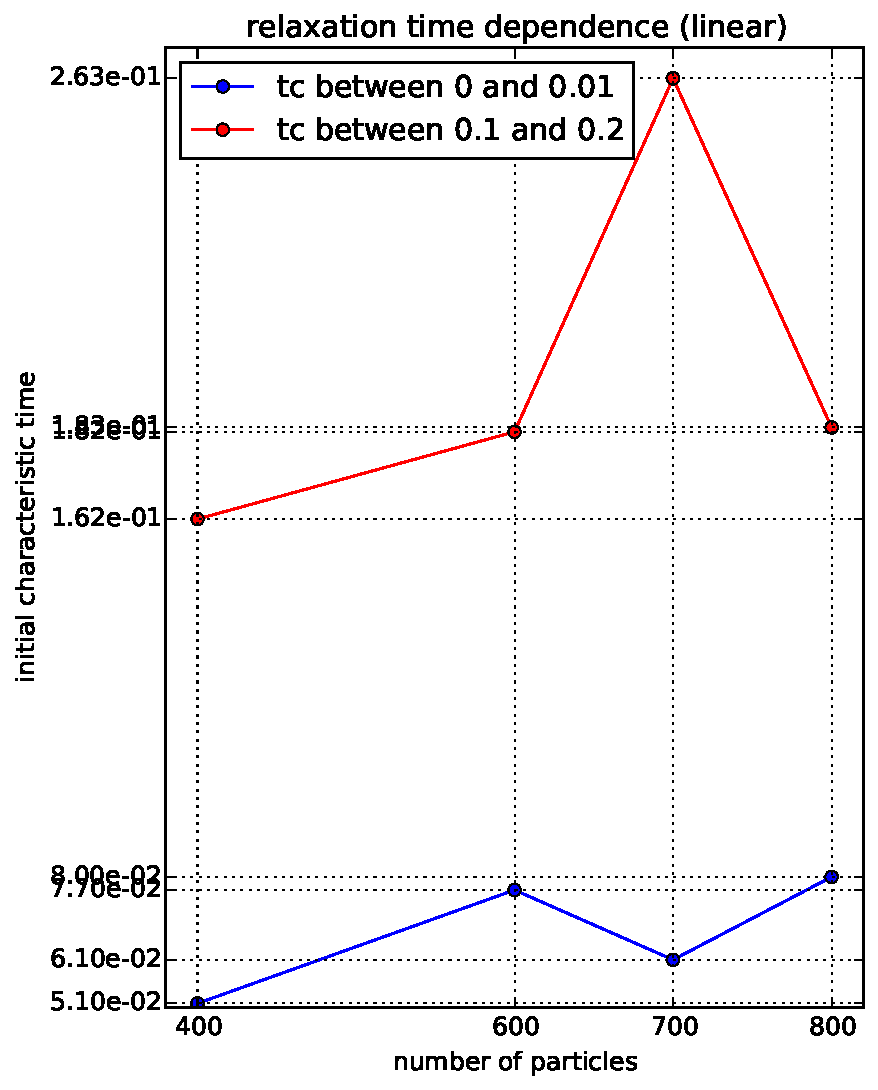
\includegraphics[width=0.45\textwidth]{../relaxation_time_dependence_wrt_concentration.pdf}
    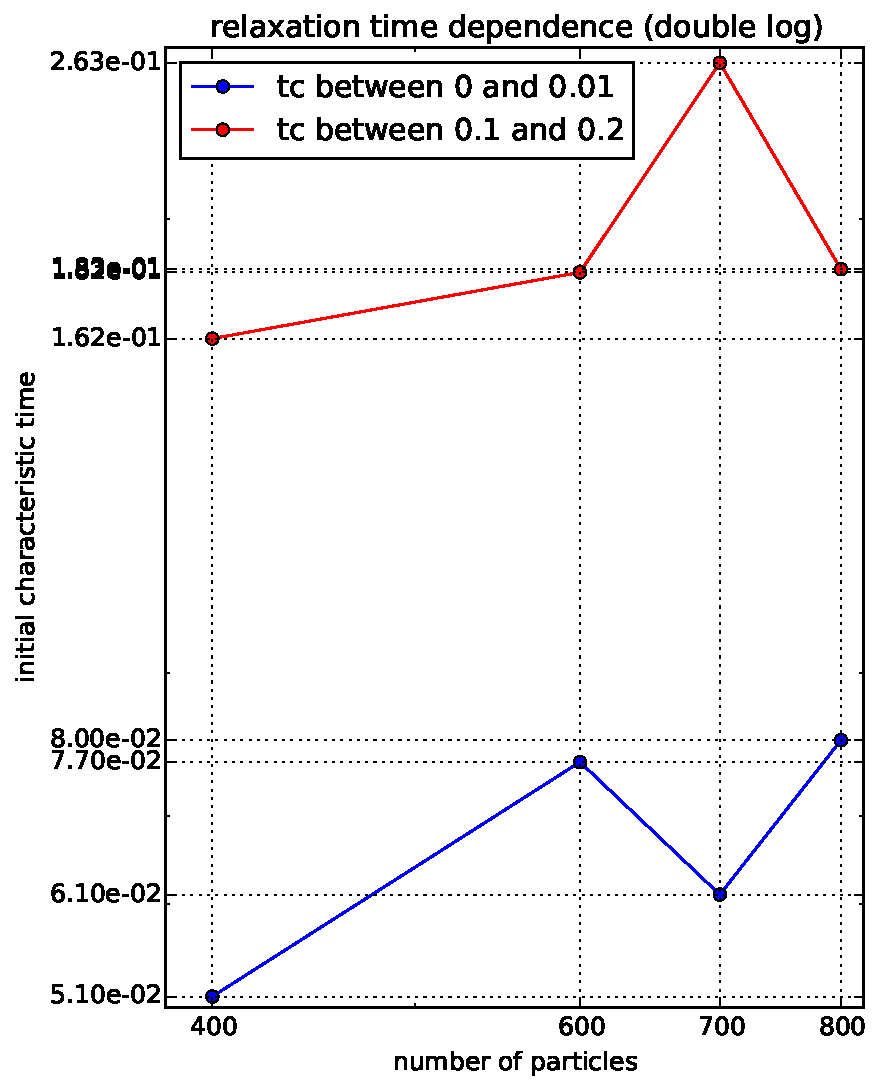
\includegraphics[width=0.45\textwidth]{../relaxation_time_dependence_wrt_concentration_loglog.pdf}
  \end{figure}
\end{frame}

% \begin{frame}
%   \frametitle<presentation>{Association Distribution ($\beta$)}
%   \begin{figure}
%     \centering
%     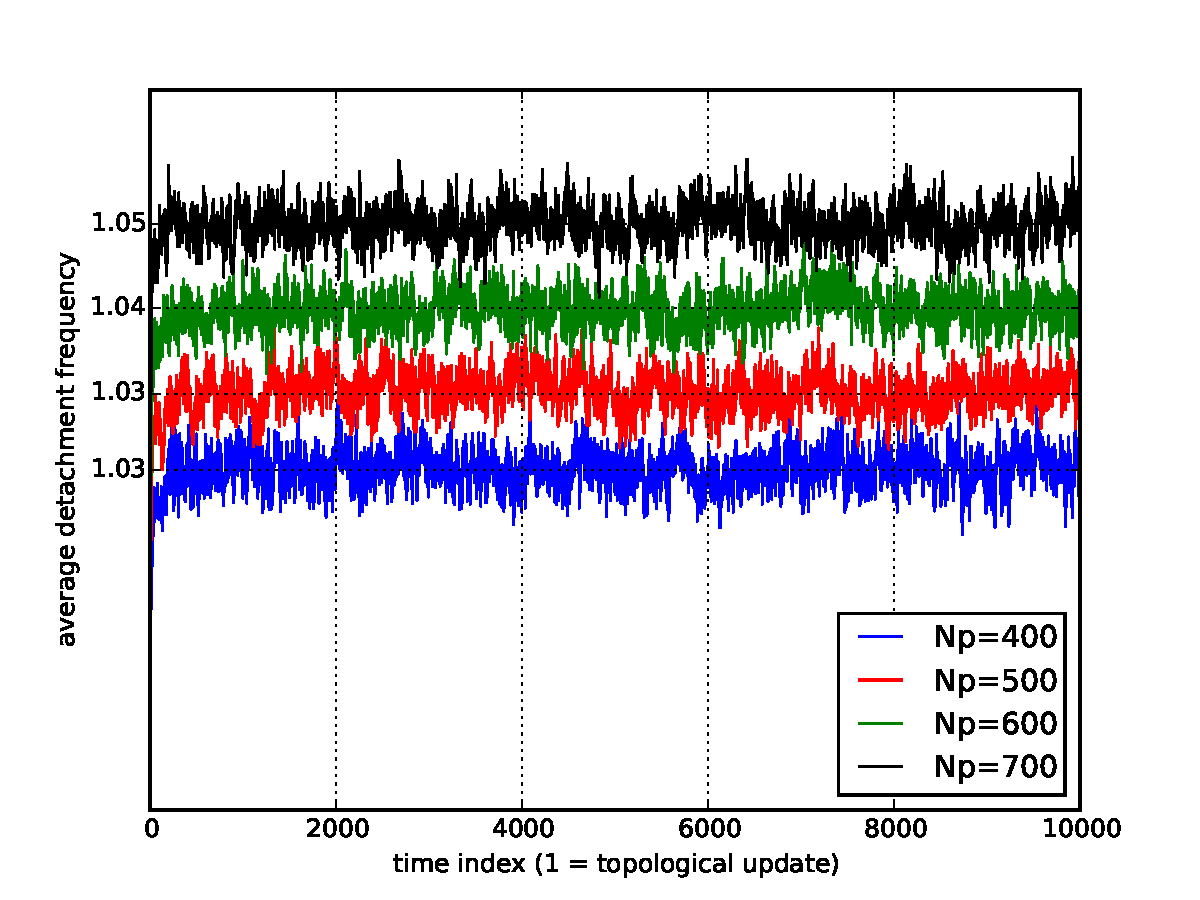
\includegraphics[width=0.45\textwidth]{../dist_beta_spectrum.pdf}
%     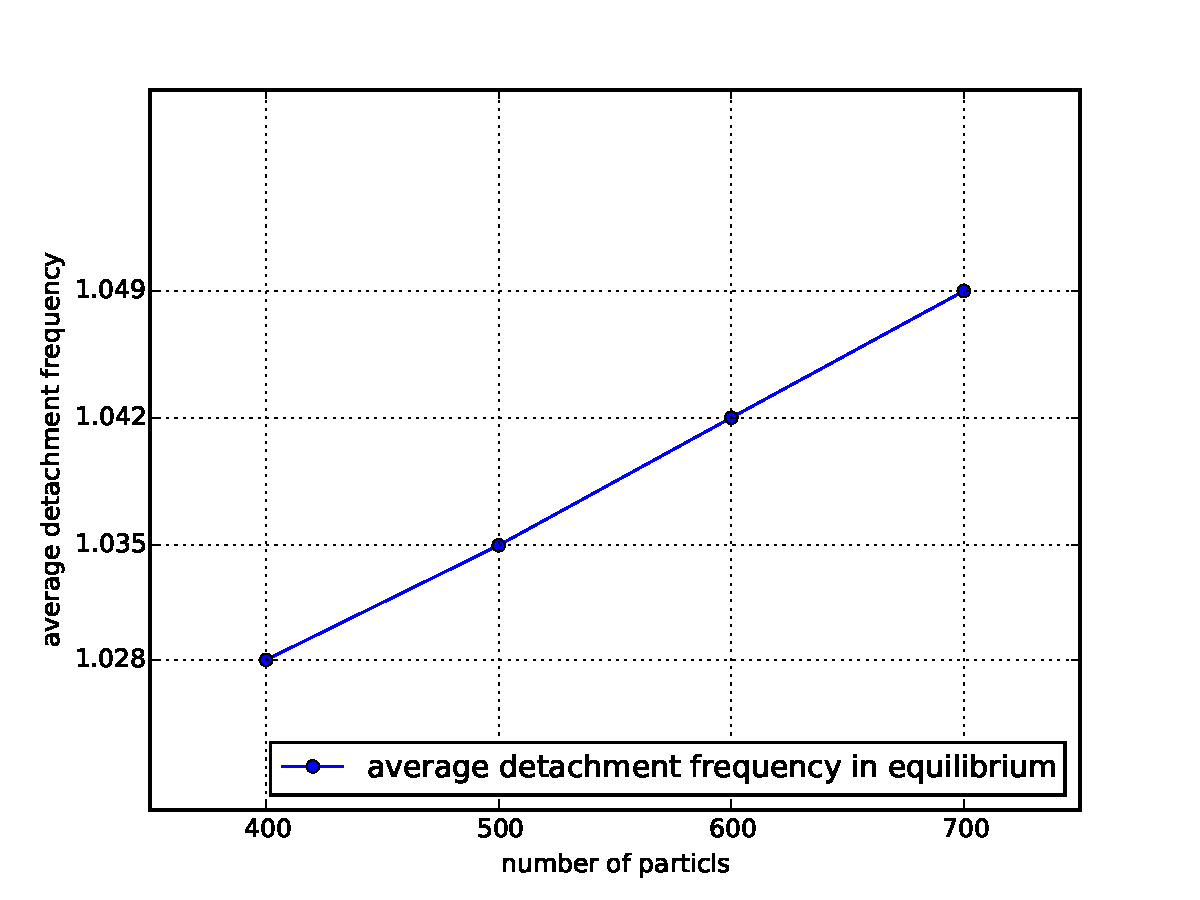
\includegraphics[width=0.45\textwidth]{../dist_beta.pdf}
%     \caption{Average detachment frequency with respect to time index for topological update (left) and its average over equilibrium time index vs. number of particles (right).}
%   \end{figure}
% \end{frame}

% \begin{frame}
%   \frametitle<presentation>{Association Distribution ($\sqrt{\langle \mathbf{r}^2\rangle}$)}
%   \begin{figure}
%     \centering
%     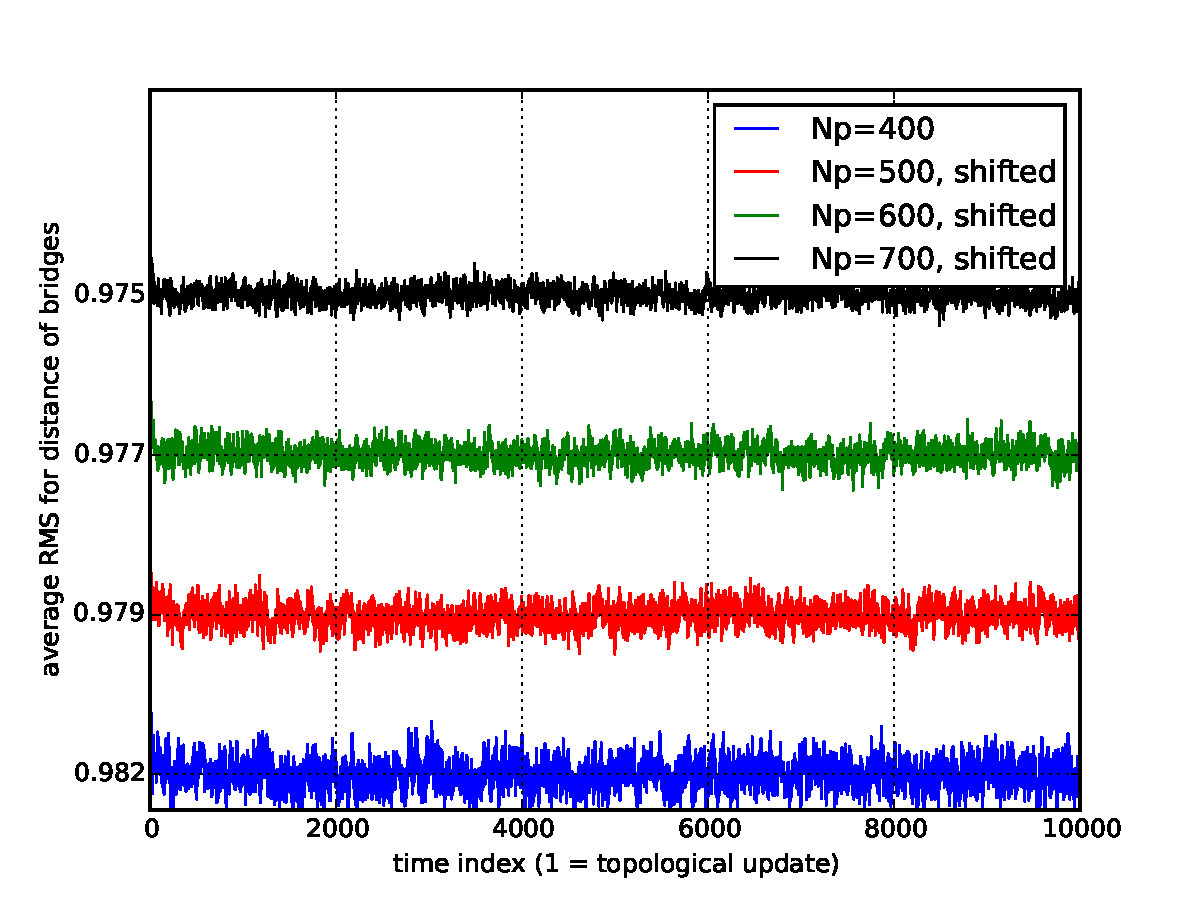
\includegraphics[width=0.45\textwidth]{../dist_Rrms_spectrum.pdf}
%     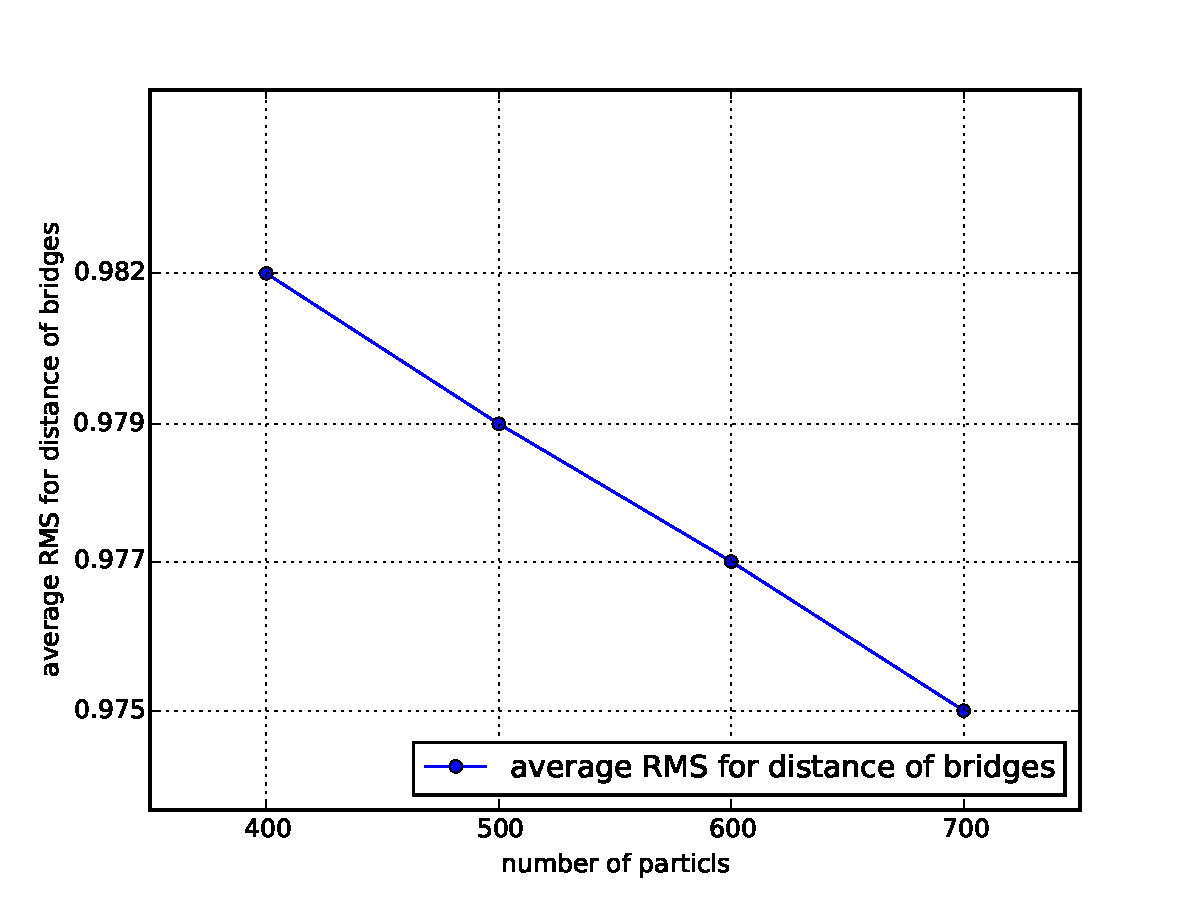
\includegraphics[width=0.45\textwidth]{../dist_Rrms.pdf}
%     \caption{Average RMS for distance of bridges with respect to time index for topological update (left) and its average over equilibrium time index vs. number of particles (right).}
%   \end{figure}

% \end{frame}


% \begin{frame}
%   \frametitle<presentation>{Equilibrium Check}
%   \begin{figure}
%     \centering
%     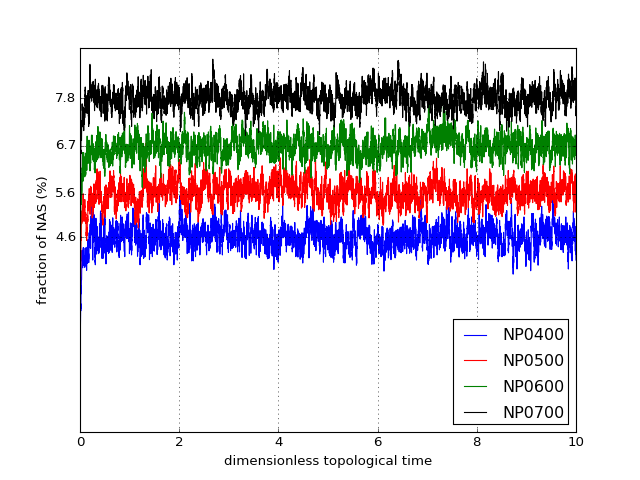
\includegraphics[height=0.8\textheight]{../NAS_check_EQ.png}
%   \end{figure}
% \end{frame}

% \begin{frame}
%   \frametitle<presentation>{Shear Stress}
%   \begin{figure}
%     \centering
%     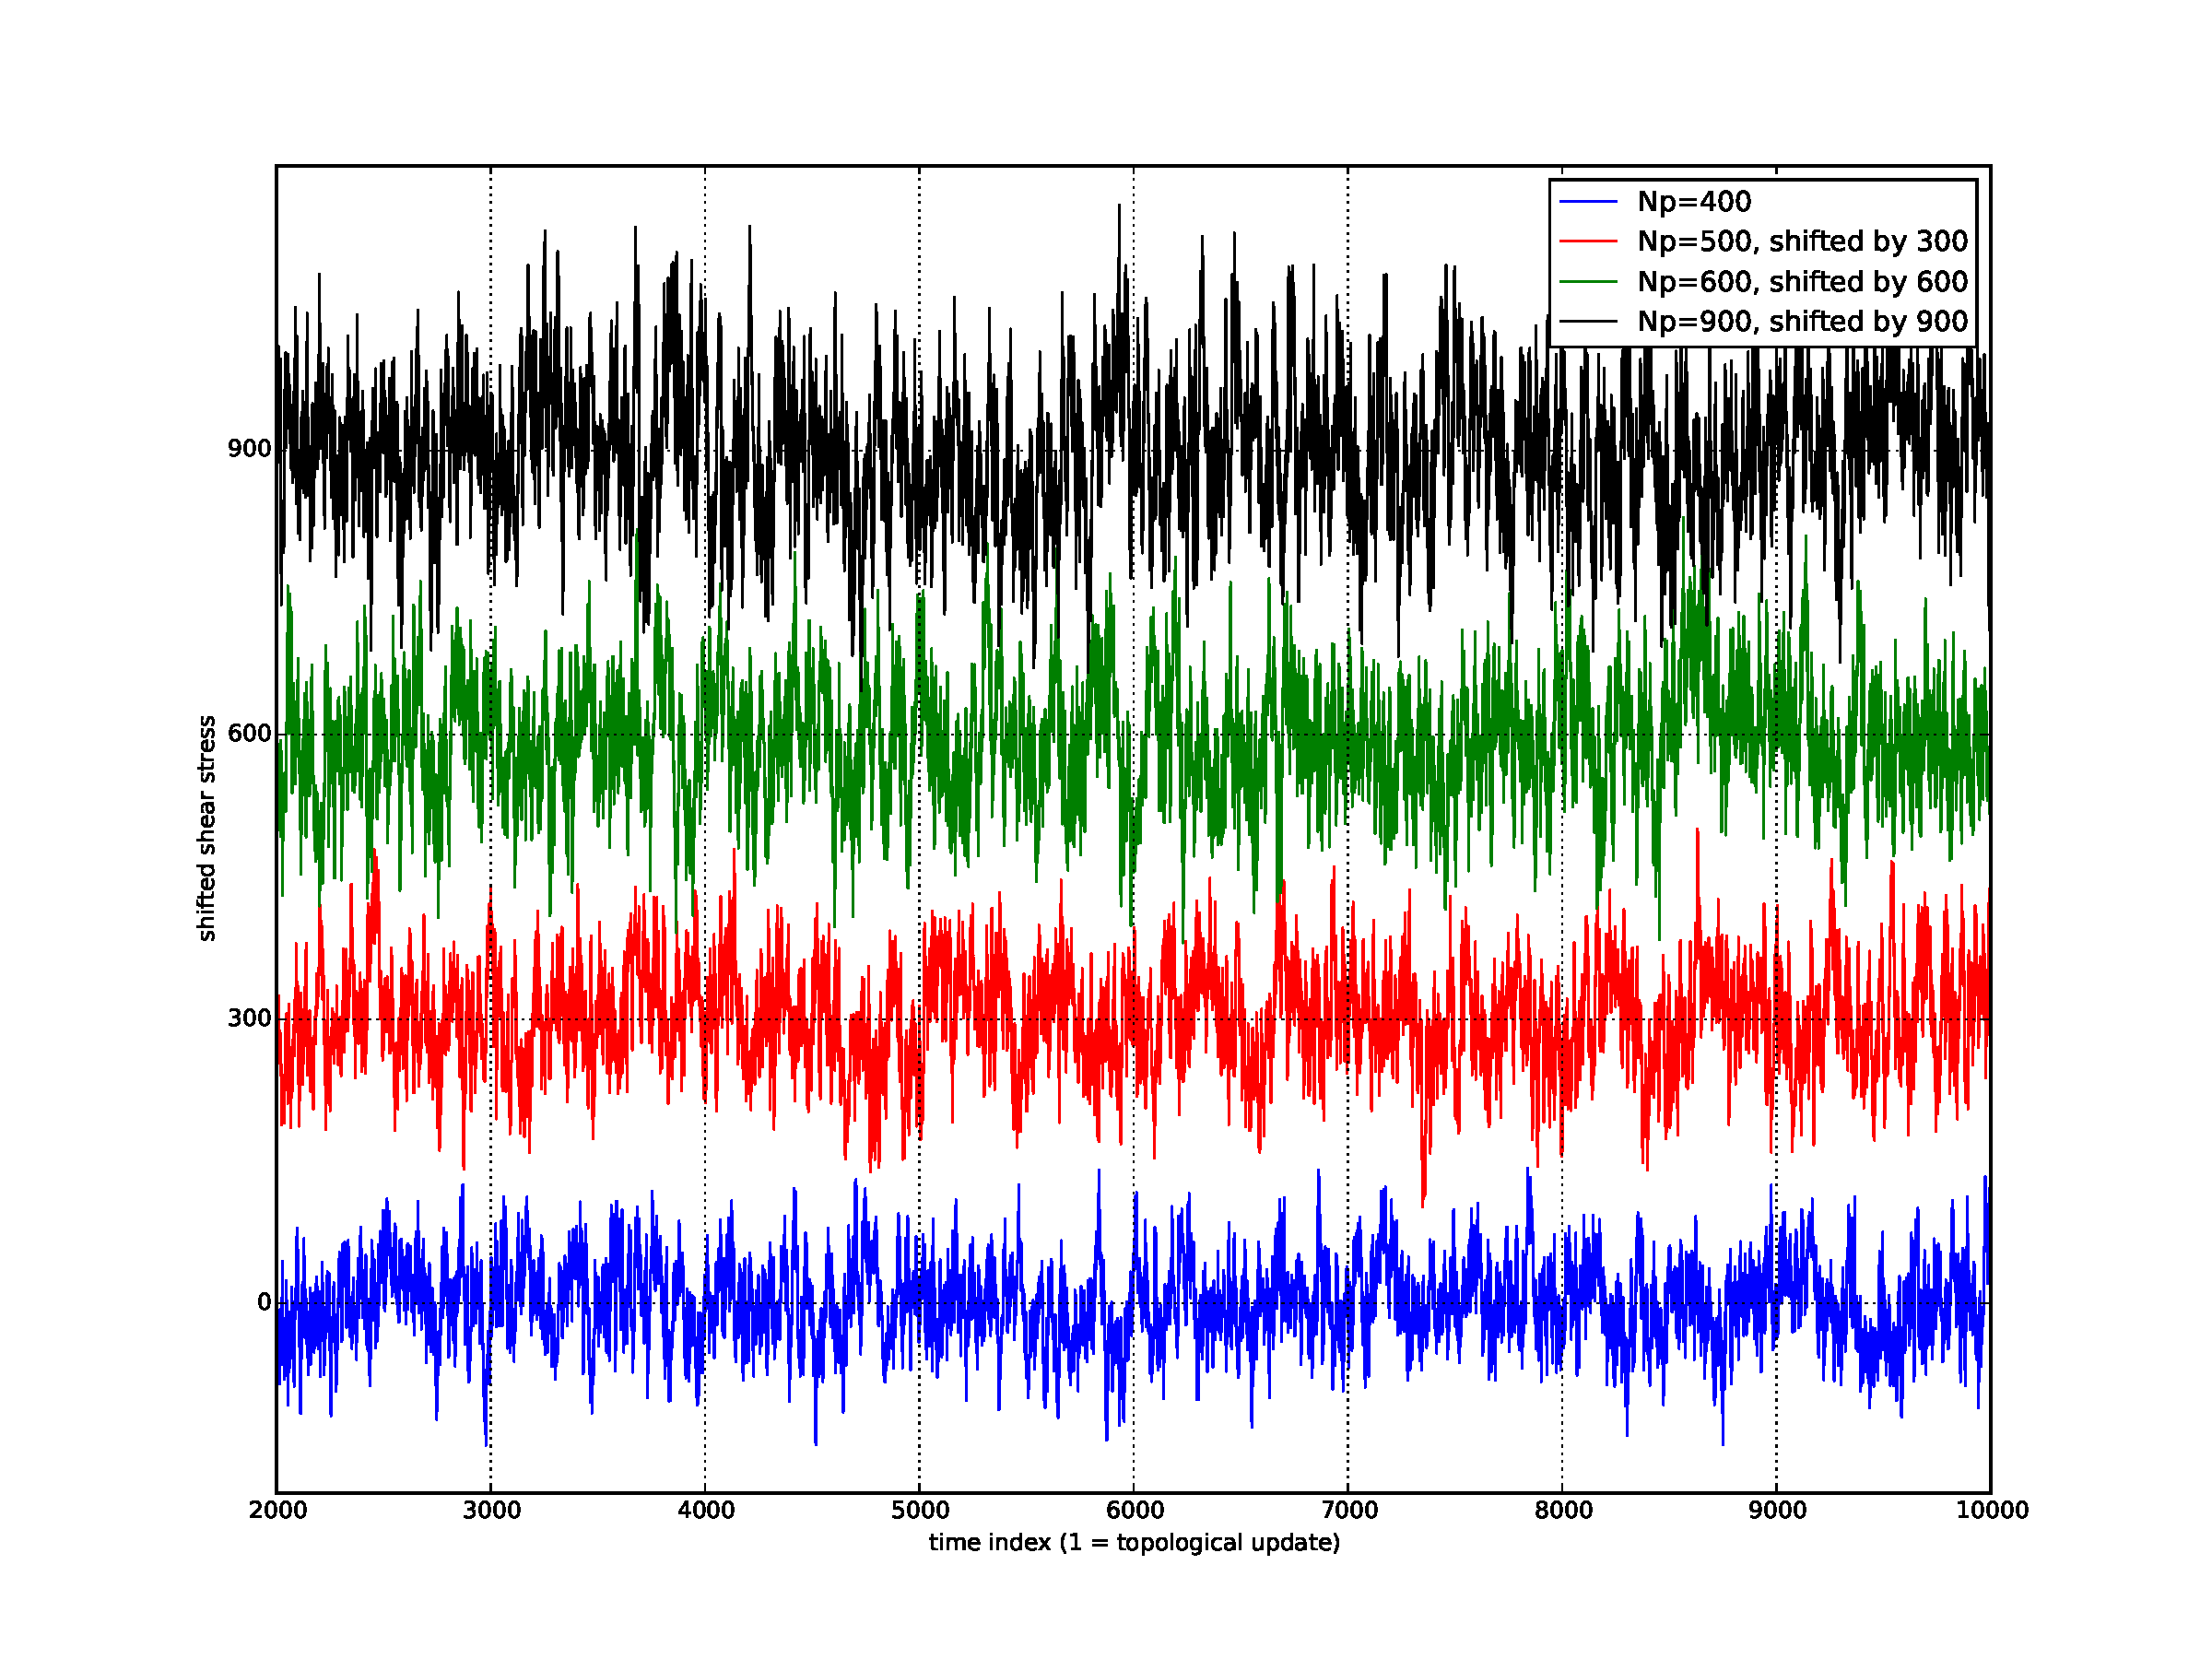
\includegraphics[height=0.8\textheight]{../tmp_shear.pdf}
%   \end{figure}
% \end{frame}

% \begin{frame}
%   \frametitle<presentation>{ACF with all time account (linear)}
%   \begin{figure}
%     \centering
%     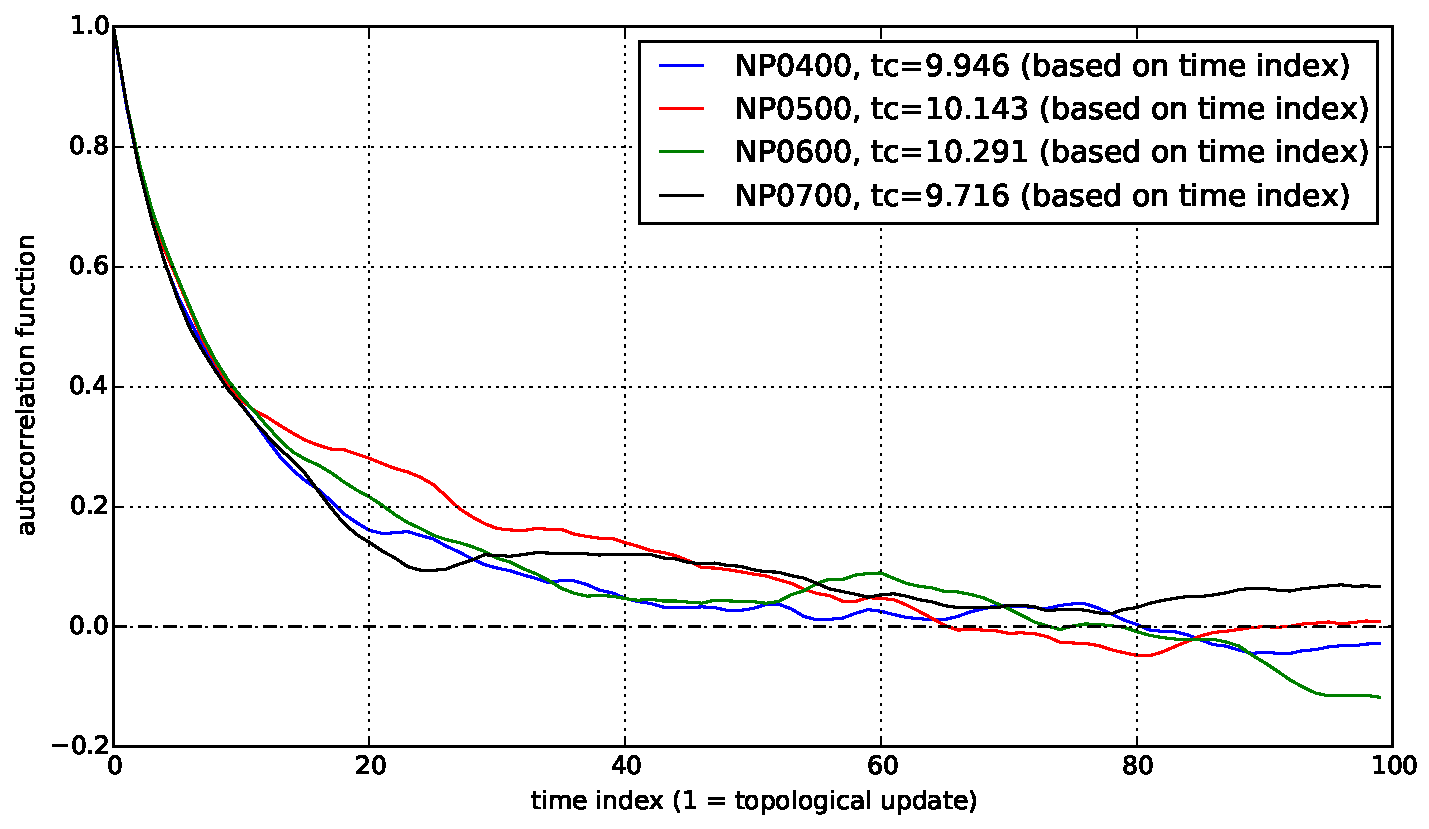
\includegraphics[height=0.75\textheight]{../ACF_all_counting_linear.pdf}
%   \end{figure}
% \end{frame}

% \begin{frame}
%   \frametitle<presentation>{ACF with all time account (semilog)}
%   \begin{figure}
%     \centering
%     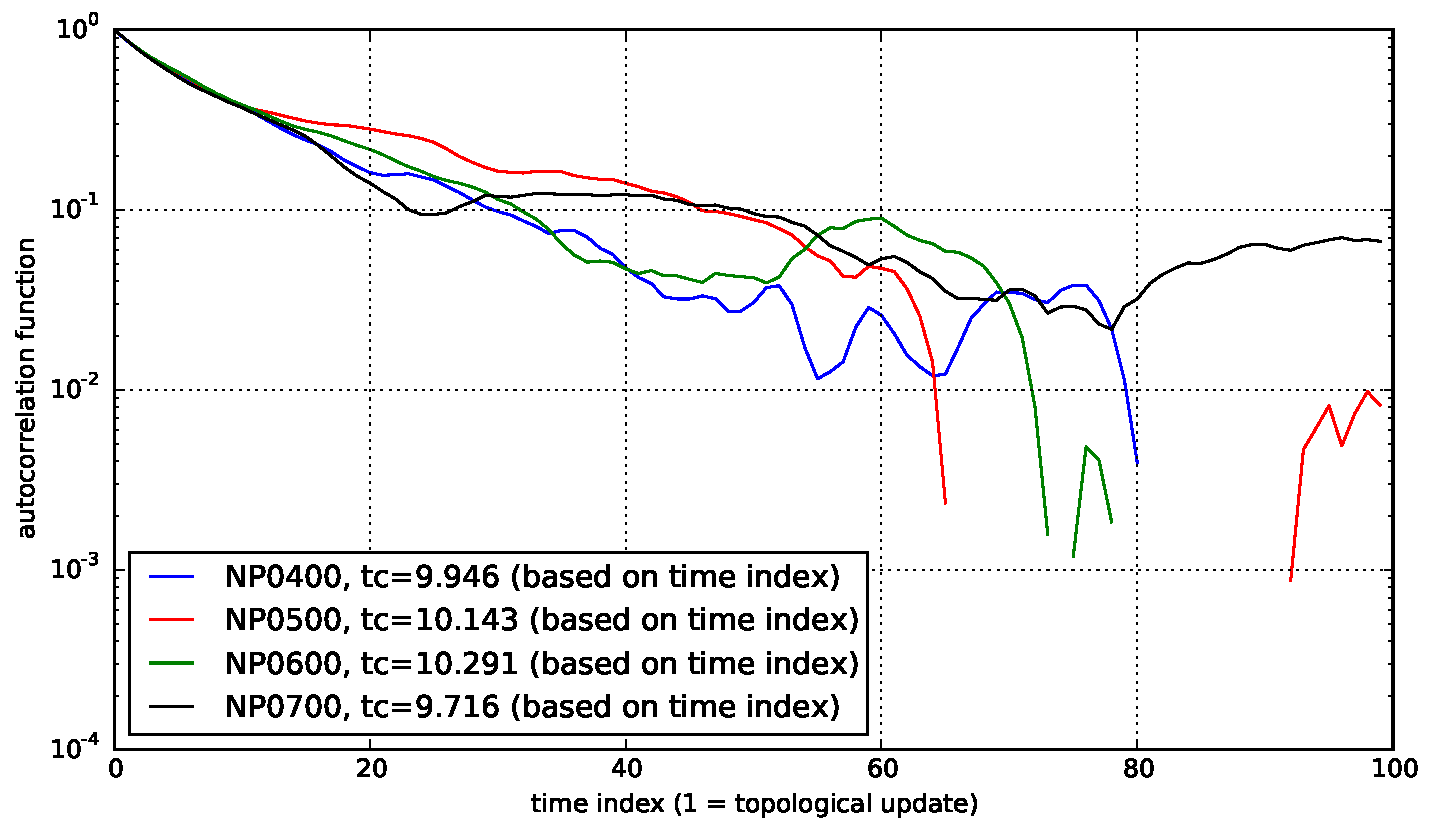
\includegraphics[height=0.75\textheight]{../ACF_all_counting_semilogy.pdf}
%   \end{figure}
% \end{frame}

% \begin{frame}
%   \frametitle<presentation>{Shear Stress (recall, detail)}
%   \begin{figure}
%     \centering
%     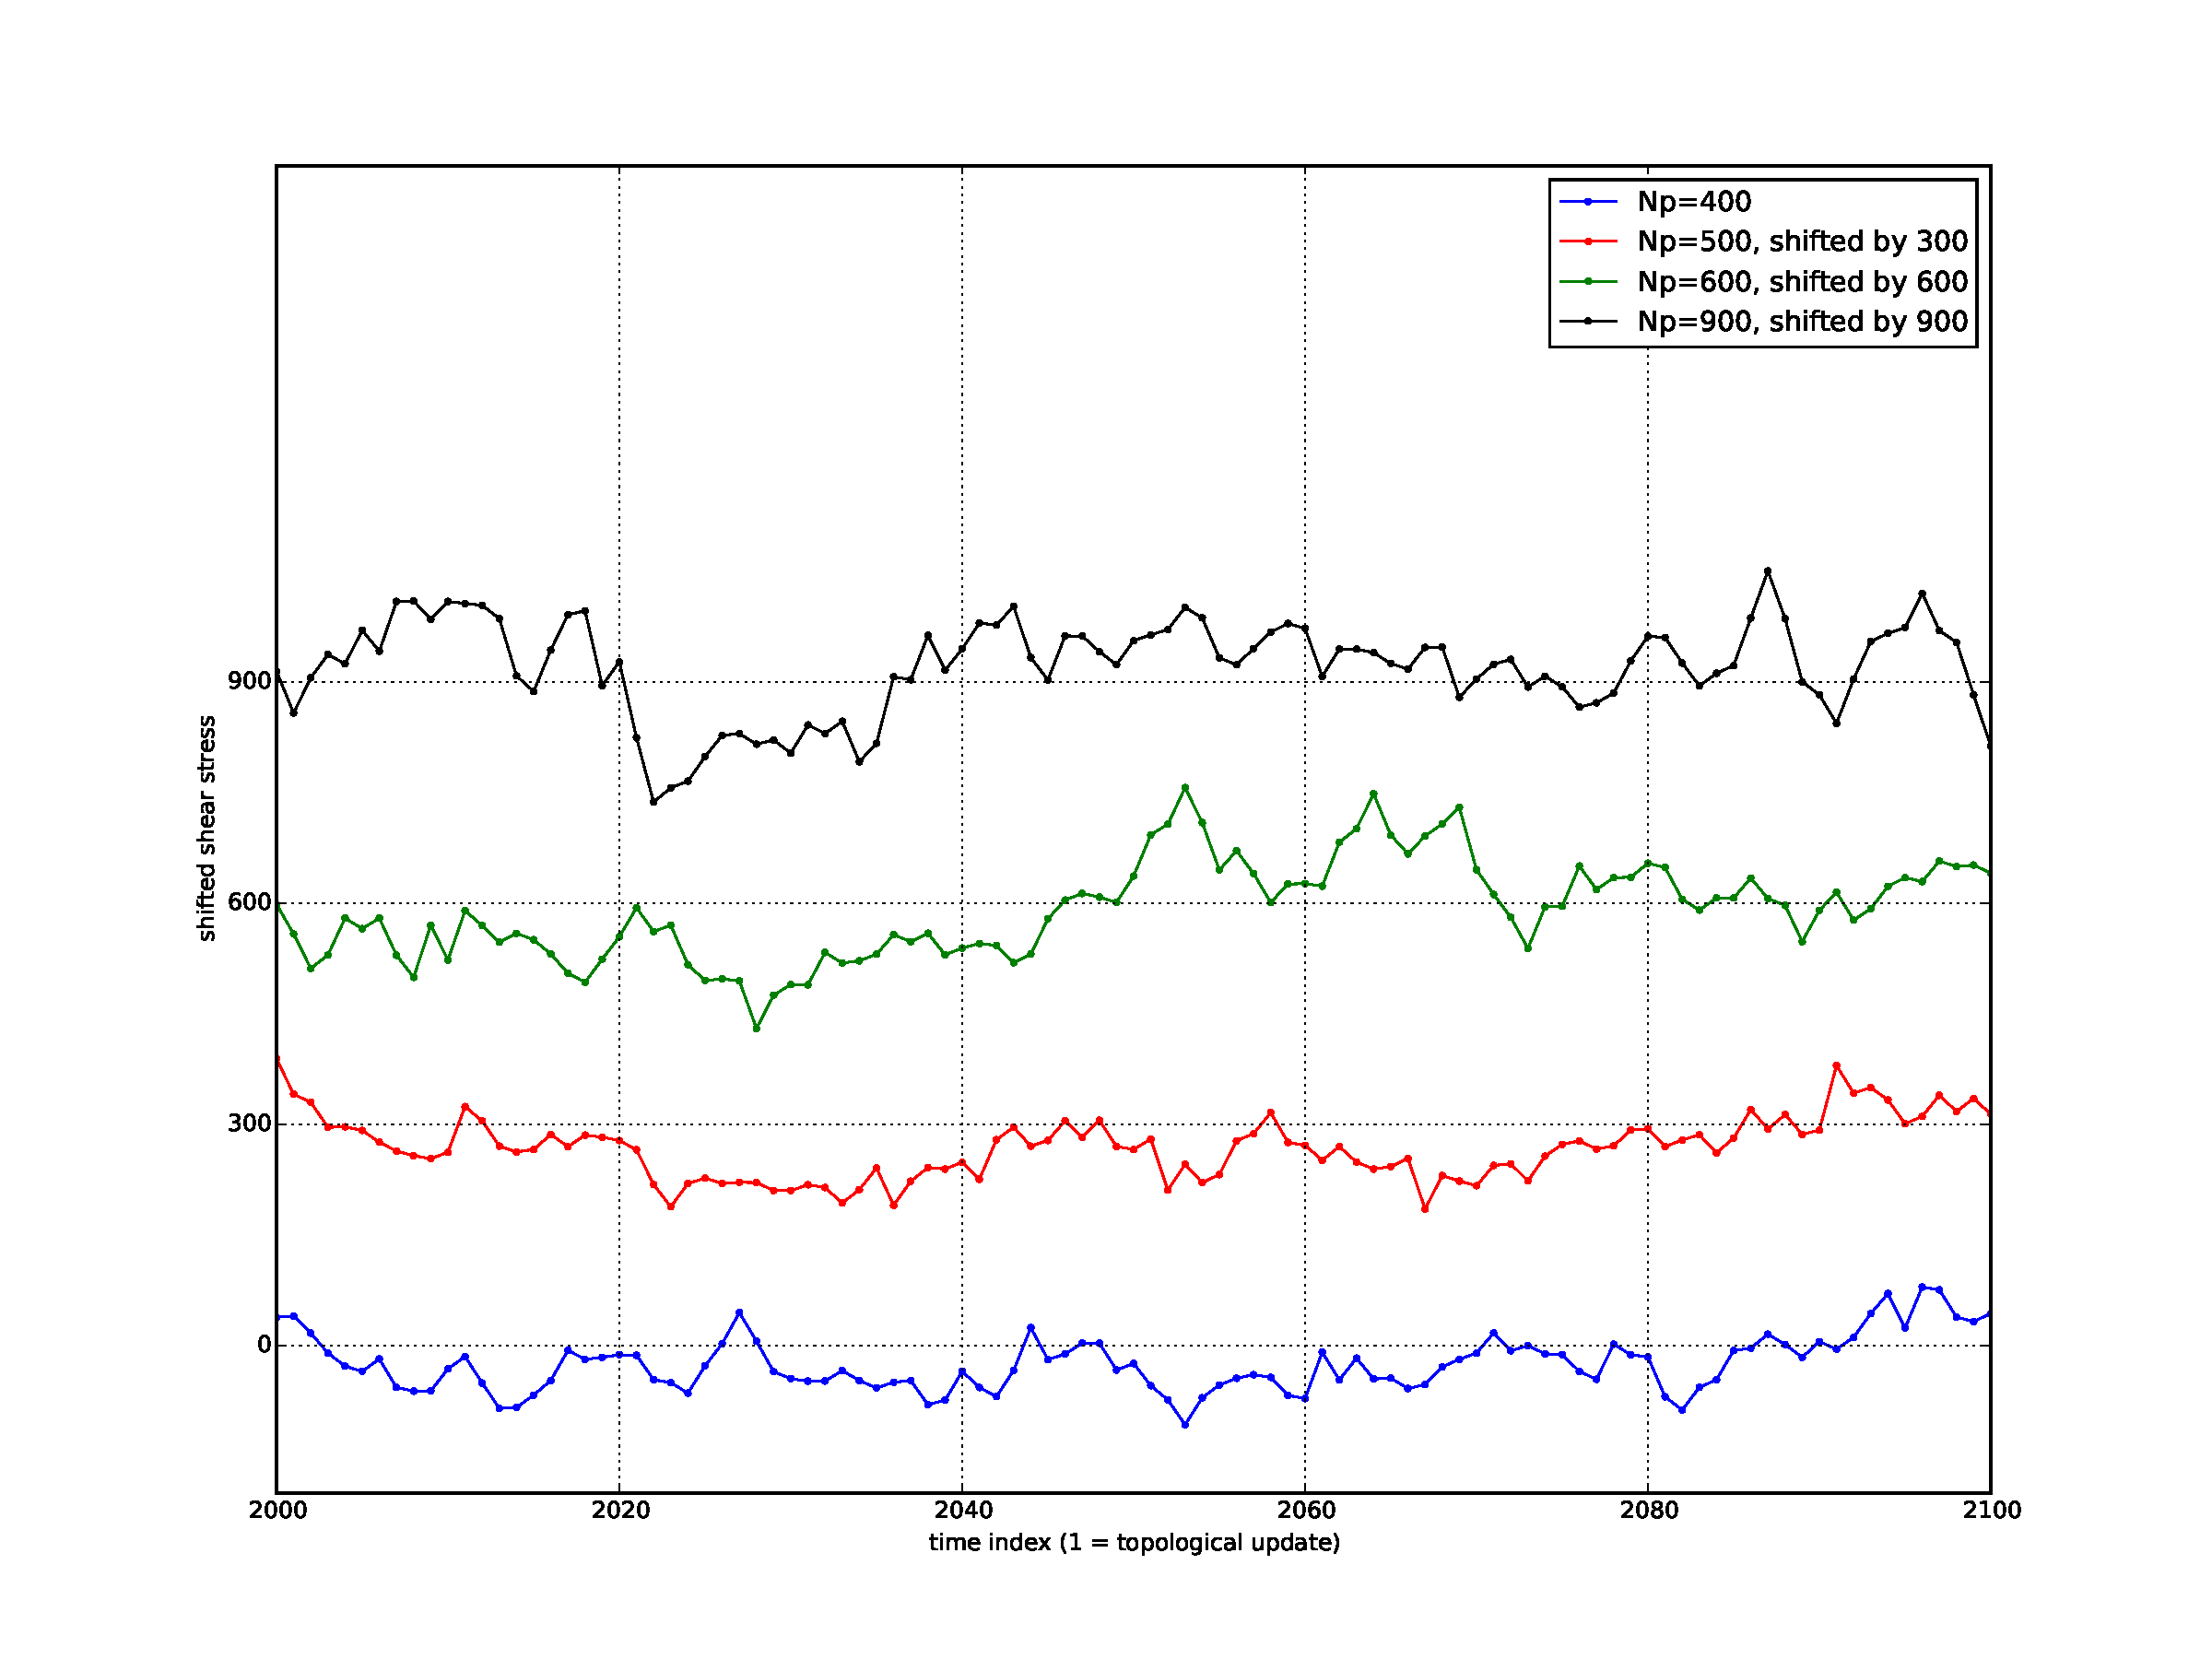
\includegraphics[height=0.8\textheight]{../tmp_shear_detail.pdf}
%   \end{figure}
% \end{frame}

% \begin{frame}
%   \frametitle<presentation>{Autoregressive Models}
%   Need to study, but basics are simple: to remove short correlation. For instance, AR(1) is the autoregressive model with the first order, which means the correlation part is only depends on the previous part. The general approaches for lagged correlation function typically extract AR(1) (or AR(k) for general) mode. There is systematic protocol to treat these data.
% \end{frame}


% % \begin{frame}
% %   \frametitle<presentation>{Conclusions and Works on Progress}
% %   \begin{itemize}
% %   \item No single correlation time is observed in biased ACF
% %   \item No consistency with respect to concentration is observed in biased ACF
% %   \item In biased ACF, the time index more than 100 can be regarded as fully uncorrelated data
% %   \item For un-biased statistics, longer computation should be necessary (in progress)
% %   \end{itemize}
% % \end{frame}

\end{document}